\documentclass[11pt]{article}

\usepackage[margin=1in]{geometry}
\usepackage{microtype}
\usepackage{booktabs}
\usepackage{amsmath}
\usepackage{hyperref}
\usepackage{graphicx}
\usepackage{listings}
\usepackage{xcolor}
\usepackage{tikz}
\usetikzlibrary{positioning}
\usepackage{enumitem}

\hypersetup{
  colorlinks=true,
  linkcolor=black,
  urlcolor=blue,
  citecolor=black
}

\lstdefinestyle{prism}{
  basicstyle=\ttfamily\small,
  keywordstyle=\color{blue},
  commentstyle=\color{gray},
  stringstyle=\color{teal},
  showstringspaces=false,
  frame=single,
  xleftmargin=0.25in,
  xrightmargin=0.25in,
  aboveskip=0.6em,
  belowskip=0.6em
}

\title{Prism: Declarative Deconstruction\\Final Report}
\author{Krishna Mula \and Kushagra Bainsla \and Tejas Chakkarwar}
\date{}

\renewenvironment{abstract}{%
  \par\noindent\textbf{Abstract}\par\noindent\normalsize
}{\par}

\begin{document}
\maketitle

\begin{abstract}
Prism is a small programming language implemented in Haskell for CS252. The language blends a minimal imperative core with functional features: user-defined functions, immutable lists, and first-class pattern matching. The key goal is ``declarative deconstruction,'' which means processing recursive data structures without manual loops or index bookkeeping. This report describes the language design, interpreter architecture, and evaluation through example programs and tests. We emphasize clear syntax, predictable semantics, and safe execution with structured error handling.
\end{abstract}

\section{Introduction and Motivation}
Processing recursive data structures in imperative languages often requires loops, indices, and nested conditionals that are verbose and error-prone. Functional languages offer pattern matching but can be less accessible to beginners. Prism bridges the gap with a small, approachable language that keeps imperative sequencing while adding expressive pattern matching.

The language is motivated by tasks where data shape matters more than control flow: symbolic manipulation, configuration logic, and rule engines. Prism programs focus on describing structure rather than iteration, which reduces accidental complexity and improves readability.

\section{Language Overview}
Prism programs consist of function definitions followed by a main expression. The syntax is intentionally compact and familiar.

\subsection{Core Features}
\begin{itemize}[leftmargin=1.2em]
  \item Integers and booleans.
  \item Variables, assignment, and sequencing with \texttt{;}
  \item Conditionals as expressions.
  \item User-defined functions with recursion.
  \item Lists and list literals.
  \item Pattern matching as a first-class expression.
\end{itemize}

\subsection{Example}
\begin{lstlisting}[style=prism]
fun length(xs) =
  match xs with
  | [] -> 0
  | h:t -> 1 + length(t)

x = [1, 2, 3, 4];
length(x)
\end{lstlisting}

\subsection{Syntax Summary}
Table~\ref{tab:syntax} summarizes the main constructs.

\begin{table}[h]
\centering
\begin{tabular}{ll}
\toprule
Construct & Example \\
\midrule
Literal & \texttt{42}, \texttt{true}, \texttt{[]} \\
List & \texttt{[1, 2, 3]} \\
Cons & \texttt{h : t} \\
Assignment & \texttt{x = 5} \\
Sequence & \texttt{x = 5; y = x + 1} \\
Conditional & \texttt{if c then e1 else e2} \\
Function & \texttt{fun f(x) = x + 1} \\
Match & \texttt{match xs with | [] -> 0 | h:t -> h} \\
\bottomrule
\end{tabular}
\caption{Core syntax constructs in Prism.}
\label{tab:syntax}
\end{table}

\section{Design Decisions}
We made several design choices to keep the language simple while enabling expressive programs.

\subsection{First-Class Pattern Matching}
Pattern matching is available as an expression, not only in function definitions. This lets programmers use pattern matching anywhere a value is needed, which keeps programs concise and avoids nested \texttt{if} chains.

\subsection{Scoped Function Calls}
Function calls evaluate with a fresh local environment for parameters, layered on top of the current global variable map. Local mutations do not persist after the call. This keeps recursion predictable and avoids accidental global mutation.

\subsection{Immutable Lists with Mutable Variables}
Lists are immutable values, but variables can be reassigned. This provides an imperative feel without sacrificing safe structural sharing.

\section{Implementation}
The interpreter is implemented in Haskell with a clean separation between syntax, parsing, and evaluation.

\subsection{Architecture}
Figure~\ref{fig:pipeline} shows the execution pipeline.

\begin{figure}[h]
\centering
\resizebox{1.0\textwidth}{!}{%
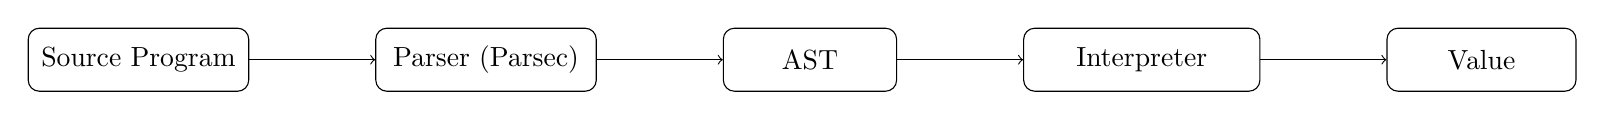
\begin{tikzpicture}[node distance=1.6cm, every node/.style={font=\normalsize}]
  \node[draw, rounded corners, align=center, minimum width=2.8cm, minimum height=0.8cm] (src) {Source Program};
  \node[draw, rounded corners, align=center, right=of src, minimum width=2.8cm, minimum height=0.8cm] (parser) {Parser (Parsec)};
  \node[draw, rounded corners, align=center, right=of parser, minimum width=2.2cm, minimum height=0.8cm] (ast) {AST};
  \node[draw, rounded corners, align=center, right=of ast, minimum width=3.0cm, minimum height=0.8cm] (interp) {Interpreter};
  \node[draw, rounded corners, align=center, right=of interp, minimum width=2.4cm, minimum height=0.8cm] (out) {Value};
  \draw[->] (src) -- (parser);
  \draw[->] (parser) -- (ast);
  \draw[->] (ast) -- (interp);
  \draw[->] (interp) -- (out);
\end{tikzpicture}%
}
\caption{Prism pipeline: source code is parsed into an AST and evaluated by the interpreter.}
\label{fig:pipeline}
\end{figure}

\subsection{AST and Values}
The AST includes expressions for literals, variables, binary operations, assignments, sequencing, function calls, list operations, and pattern matching. Runtime values include integers, booleans, and lists. Functions are stored in a separate function environment rather than as first-class values.

\subsection{Interpreter State and Error Handling}
Evaluation uses a monad stack: \texttt{ExceptT String (State InterpreterState)}. The state stores the variable environment and function environment. Errors like unbound variables, division by zero, and pattern match failure are reported without crashing the host program.

\subsection{Pattern Matching}
Pattern matching checks patterns in order and returns bindings when a match succeeds. Supported patterns are variables, literals, empty list, cons patterns, and a wildcard. Binding results are merged into the environment before evaluating the matching branch.

\begin{figure}[h]
\centering
\resizebox{0.6\textwidth}{!}{%
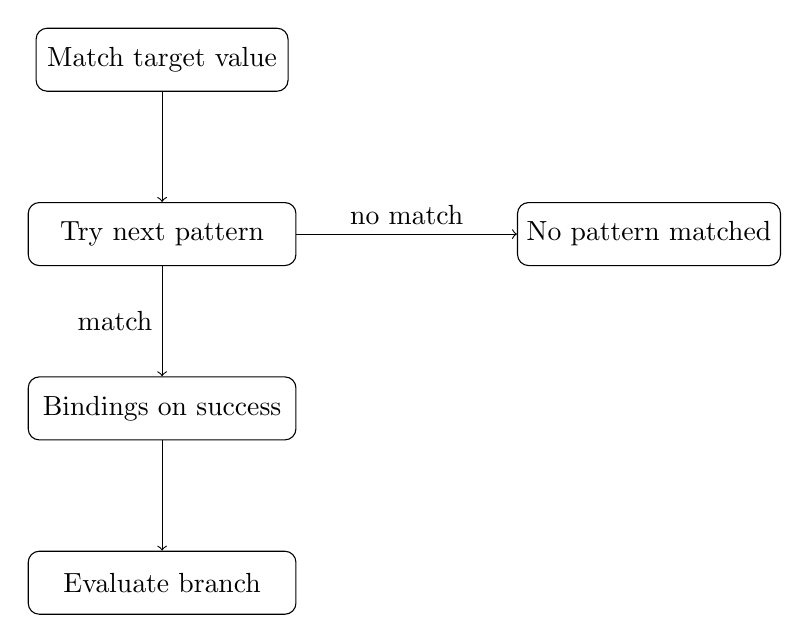
\begin{tikzpicture}[node distance=1.4cm, every node/.style={font=\normalsize}]
  \node[draw, rounded corners, align=center, minimum width=3.2cm, minimum height=0.8cm] (start) {Match target value};
  \node[draw, rounded corners, align=center, below=of start, minimum width=3.4cm, minimum height=0.8cm] (try) {Try next pattern};
  \node[draw, rounded corners, align=center, below=of try, minimum width=3.4cm, minimum height=0.8cm] (bind) {Bindings on success};
  \node[draw, rounded corners, align=center, right=2.8cm of try, minimum width=3.2cm, minimum height=0.8cm] (fail) {No pattern matched};
  \node[draw, rounded corners, align=center, below=of bind, minimum width=3.4cm, minimum height=0.8cm] (eval) {Evaluate branch};
  \draw[->] (start) -- (try);
  \draw[->] (try) -- node[left]{match} (bind);
  \draw[->] (try) -- node[above]{no match} (fail);
  \draw[->] (bind) -- (eval);
\end{tikzpicture}%
}
\caption{Pattern matching flow in the interpreter.}
\label{fig:match}
\end{figure}

\section{Evaluation and Testing}
We tested the interpreter using a suite of sample programs in the \texttt{test} directory. These cover recursion, list operations, mutation, error handling, and pattern matching.

\subsection{Test Programs}
\begin{itemize}[leftmargin=1.2em]
  \item \texttt{demo.lp}: end-to-end demo with recursive functions and list processing.
  \item \texttt{recursion\_test.lp}: factorial and Fibonacci recursion.
  \item \texttt{list\_ops.lp}: list construction, reverse, and mapping examples.
  \item \texttt{mutability\_test.lp}: assignment and sequencing behavior.
  \item \texttt{data\_deconstruction.lp}: list-processing pipeline with pattern matching.
  \item \texttt{error\_cases.lp}: safe division plus commented examples for runtime errors.
\end{itemize}

\subsection{Observations}
The interpreter successfully evaluates all valid programs and reports clear errors for invalid ones. Pattern matching significantly reduces boilerplate for recursive list programs compared to traditional loop-based approaches. The static pre-check for unbound variables catches common mistakes before execution.

\section{Limitations and Future Work}
Prism currently lacks a type system and advanced data structures beyond lists. Error messages are descriptive but do not include full stack traces. Future work could include:
\begin{itemize}[leftmargin=1.2em]
  \item A lightweight static type checker.
  \item Better source-position reporting for runtime errors.
  \item Additional data structures (records or algebraic data types).
  \item Optimizations such as tail-call optimization or lazy evaluation.
\end{itemize}

\section{Conclusion}
Prism demonstrates that a small language can still deliver expressive, high-level features. By combining an imperative core with functional pattern matching, Prism supports concise programs for recursive data and offers clean, predictable execution semantics. The Haskell implementation provides clarity and safety while remaining accessible for educational use.

\begin{thebibliography}{9}
\bibitem{parsec}
Daan Leijen. \textit{Parsec: Direct Style Monadic Parser Combinators for the Real World}. Department of Computer Science, Utrecht University, 2001. Accessed April 26, 2026.

\bibitem{haskell2010}
Simon Marlow (ed.). \textit{Haskell 2010 Language Report}. 2010. \url{https://www.haskell.org/onlinereport/haskell2010/}. Accessed April 26, 2026.

\bibitem{cleancode}
Robert C. Martin. \textit{Clean Code: A Handbook of Agile Software Craftsmanship}. Prentice Hall, 2008.

\bibitem{designbycontract}
Bertrand Meyer. ``Applying Design by Contract.'' \textit{IEEE Computer}, 25(10): 40--51, 1992. Accessed April 26, 2026.

\bibitem{craftofhaskell}
Simon Thompson. \textit{Haskell: The Craft of Functional Programming} (3rd ed.). Addison-Wesley, 2011.
\end{thebibliography}

\end{document}
